%  25 Oct 2024 21:59:44
\documentclass{article}
\usepackage{geometry,booktabs,longtable,pdflscape,rotating,threeparttable,subfigure,graphicx,}
\usepackage{tabularx,xcolor,colortbl,}
\usepackage{hyperref}
\hypersetup{                           colorlinks=true,                   linkcolor={blue!50!black},                    filecolor={blue!50!black},                 urlcolor={blue!80!black},                     }                              \date{}
\geometry{verbose,letterpaper,lmargin=2.5cm,tmargin=2.5cm}

\begin{document}

\title{A descriptive analysis of the auto.dta data}
\maketitle
\section{Introduction}
This file provides examples of the use of the latexlog package.
The data used in this example is the auto.dta data set, which is a sample data set provided with Stata.
\section{Summary Statistics}
\begin{figure}[h] 
\centering 
\begin{tabular}{p{6in}}
\caption{A scatterplot of price vs. weight using the addfig subcommand} 
\end{tabular}
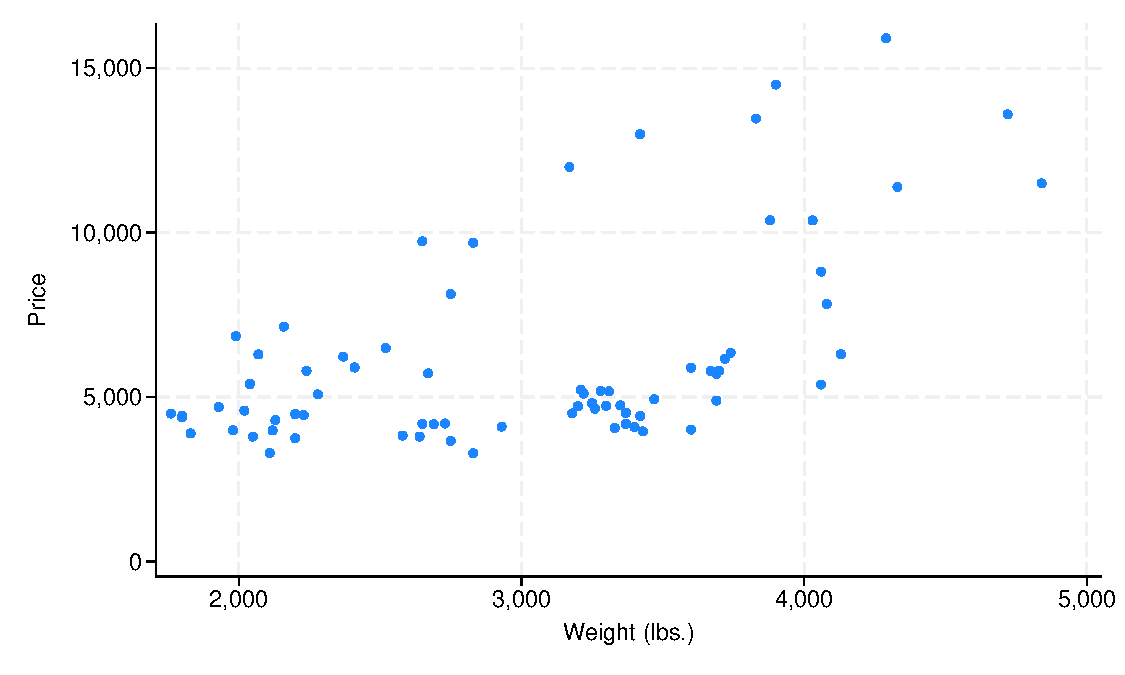
\includegraphics[width = .8\textwidth]{scatter_price.pdf} \\ 
\begin{tabular}{p{6in}}  
\footnotesize \vspace{2pt} 
\centering \textbf{Notes:} Based on the auto.dta data 
\end{tabular} 
\end{figure} 
\begin{figure}[h] 
\centering 
\begin{tabular}{p{6in}}
\caption{Four Scatterplots of different variables vs. weight using the subfigure subcommand} 
\end{tabular}
\subfigure[Price vs. weight]{
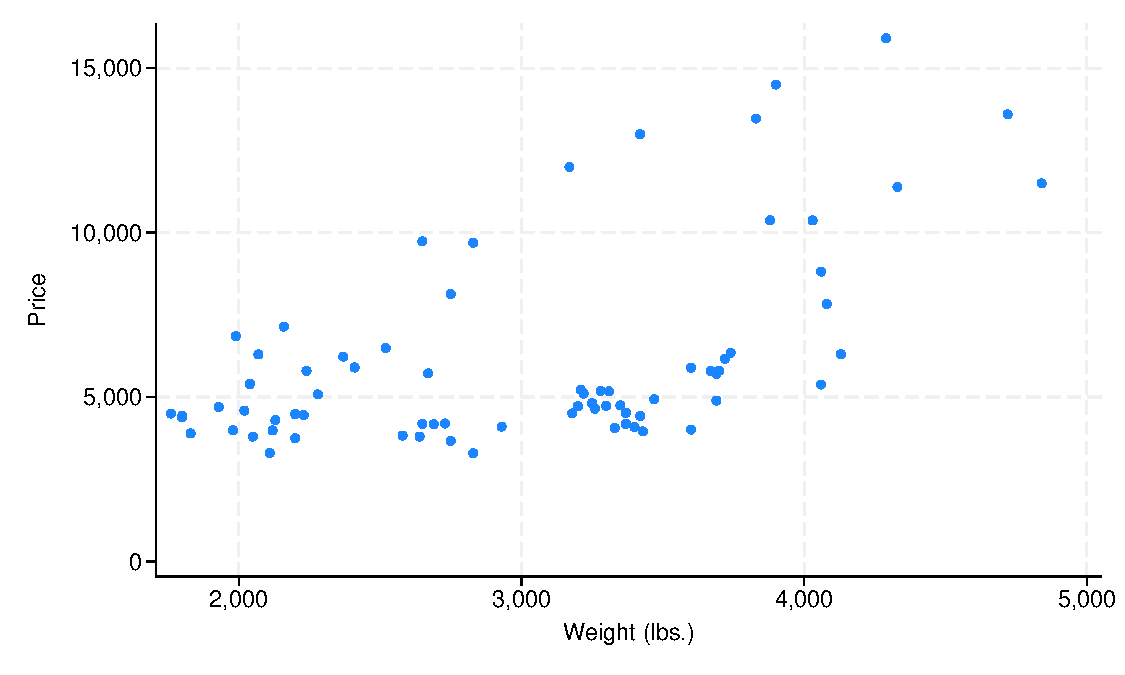
\includegraphics[clip=true, tim=0 0 0 0, width = .4\textwidth]{scatter_price.pdf} \\ 
}
\subfigure[Gear ratio vs. weight]{
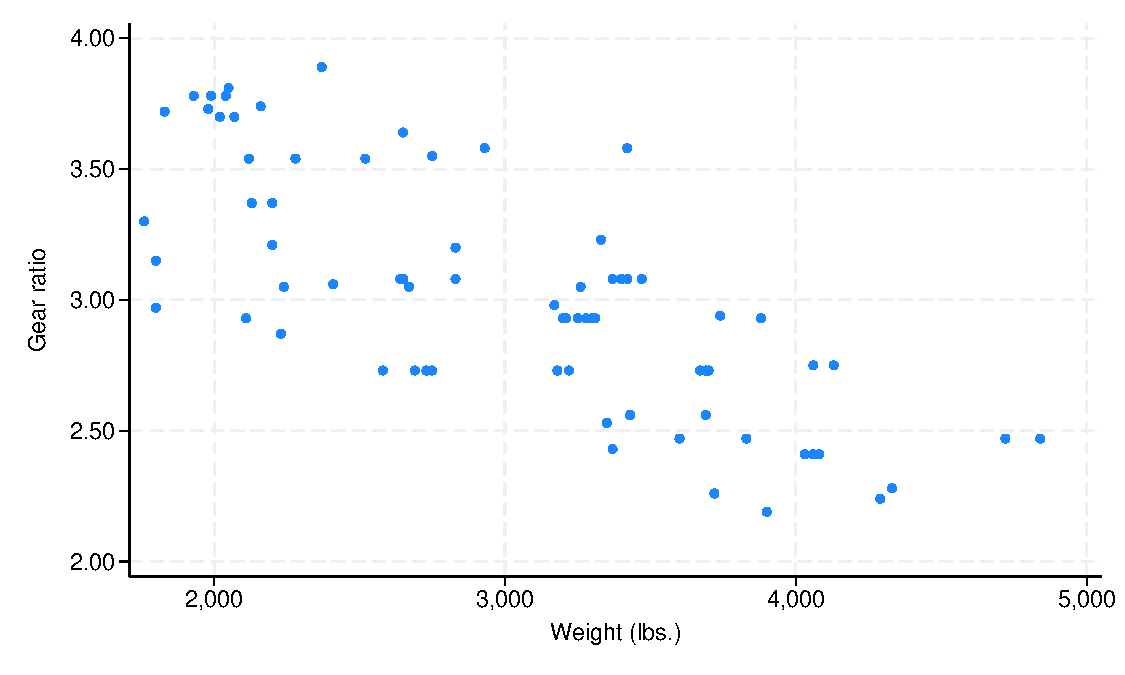
\includegraphics[clip=true, tim=0 0 0 0, width = .4\textwidth]{scatter_gear_ratio.pdf} \\ 
}
\subfigure[Trunk space (cu. ft.) vs. weight]{
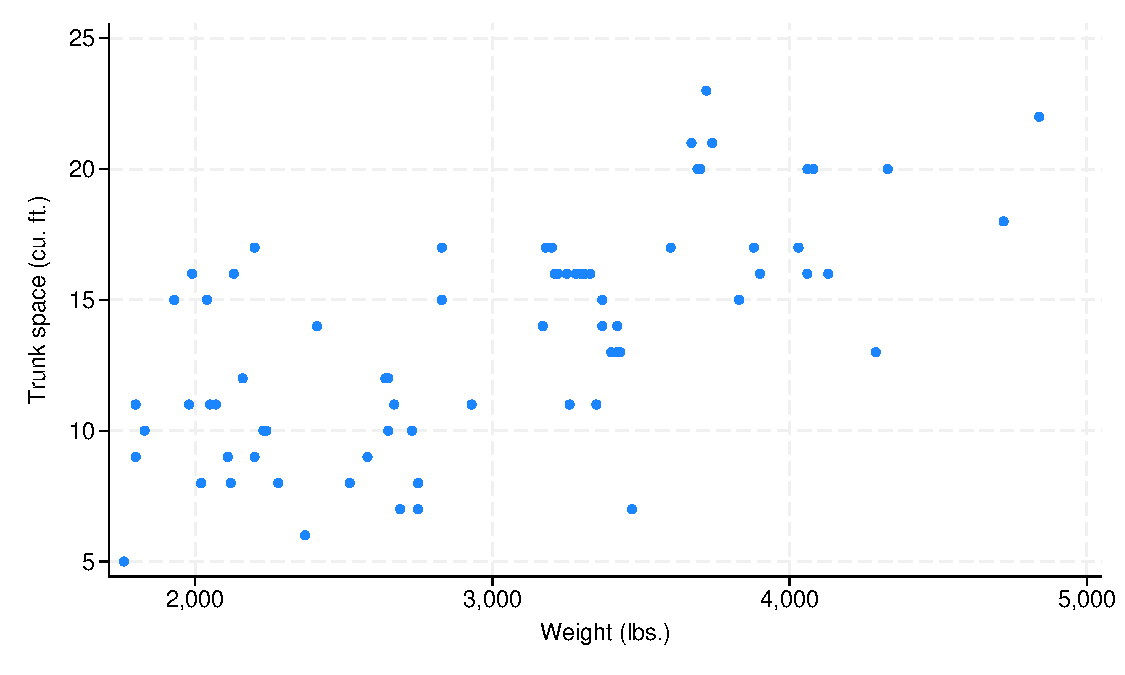
\includegraphics[clip=true, tim=0 0 0 0, width = .4\textwidth]{scatter_trunk.pdf} \\ 
}
\subfigure[Displacement (cu. in.) vs. weight]{
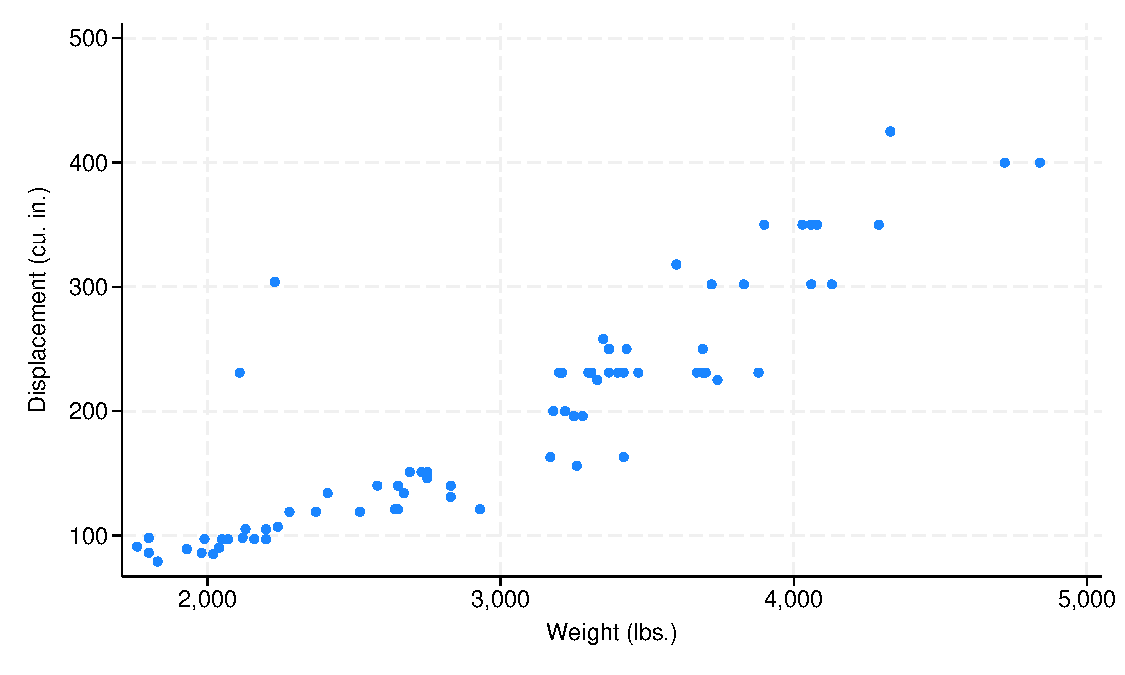
\includegraphics[clip=true, tim=0 0 0 0, width = .4\textwidth]{scatter_displacement.pdf} \\ 
}
\begin{tabular}{p{6in}}  
\footnotesize \vspace{2pt} 
\centering \textbf{Notes:} Based on the auto.dta data 
\end{tabular} 
\end{figure} 
\clearpage\pagebreak
\section{Saving Tables with latexlog}
Since latexlog operates directly on a tex file, it is easy to save 
tables created with the esttab command or other commands that 
produce latex output that is appended to a file.
Here is an example of saving a table created with the esttab command:
 
\vspace{10pt}
{
\def\sym#1{\ifmmode^{#1}\else\(^{#1}\)\fi}
\begin{tabular}{l*{1}{c}}
\toprule
            &\multicolumn{1}{c}{(1)}\\
            &\multicolumn{1}{c}{price}\\
\midrule
mpg         &      -238.9\sym{***}\\
            &     (-4.50)         \\
\addlinespace
\_cons      &     11253.1\sym{***}\\
            &      (9.61)         \\
\midrule
\(N\)       &          74         \\
\bottomrule
\multicolumn{2}{l}{\footnotesize \textit{t} statistics in parentheses}\\
\multicolumn{2}{l}{\footnotesize \sym{*} \(p<0.05\), \sym{**} \(p<0.01\), \sym{***} \(p<0.001\)}\\
\end{tabular}
}

\vspace{10pt}
Stata's table command is very flexible and powerful. 
The following example creates a table of the number of foreign and domestic cars 
in each MPG category using Stata's table command. 
This table is then saved to the log file using the collect export subcommand.
\begin{table}[htbp] 
\centering 
\begin{threeparttable} 
\caption{Two Way Table using Stata table command and latexlog collect export subcommand} 

\centering
\begin{tabular}{llll}
\toprule
\multicolumn{1}{c}{} &
  \multicolumn{3}{c}{MPG category} \\
\multicolumn{1}{c}{} &
  \multicolumn{1}{r}{Ineffcient} &
  \multicolumn{1}{r}{Moderate} &
  \multicolumn{1}{r}{Efficient} \\
\midrule
\multicolumn{1}{l}{Car origin} &
  \multicolumn{1}{r}{} &
  \multicolumn{1}{r}{} &
  \multicolumn{1}{r}{} \\
\multicolumn{1}{l}{\hspace{1em}Domestic} &
  \multicolumn{1}{r}{} &
  \multicolumn{1}{r}{} &
  \multicolumn{1}{r}{} \\
\multicolumn{1}{l}{\hspace{2em}Weight $>$=3000 lbs} &
  \multicolumn{1}{r}{} &
  \multicolumn{1}{r}{} &
  \multicolumn{1}{r}{} \\
\multicolumn{1}{l}{\hspace{3em}0} &
  \multicolumn{1}{r}{9} &
  \multicolumn{1}{r}{6} &
  \multicolumn{1}{r}{} \\
\multicolumn{1}{l}{\hspace{3em}1} &
  \multicolumn{1}{r}{36} &
  \multicolumn{1}{r}{1} &
  \multicolumn{1}{r}{} \\
\multicolumn{1}{l}{\hspace{1em}Foreign} &
  \multicolumn{1}{r}{} &
  \multicolumn{1}{r}{} &
  \multicolumn{1}{r}{} \\
\multicolumn{1}{l}{\hspace{2em}Weight $>$=3000 lbs} &
  \multicolumn{1}{r}{} &
  \multicolumn{1}{r}{} &
  \multicolumn{1}{r}{} \\
\multicolumn{1}{l}{\hspace{3em}0} &
  \multicolumn{1}{r}{13} &
  \multicolumn{1}{r}{6} &
  \multicolumn{1}{r}{1} \\
\multicolumn{1}{l}{\hspace{3em}1} &
  \multicolumn{1}{r}{2} &
  \multicolumn{1}{r}{} &
  \multicolumn{1}{r}{} \\
\bottomrule
\end{tabular}

\textbf{Notes:} more notes 
\end{threeparttable} 
\end{table}
\begin{table}[htbp] 
\centering 
\caption{Regression Table using Stata etable command and latexlog collect export subcommand} 

\centering
\begin{tabular}{lll}
\toprule
\multicolumn{1}{r}{} &
  \multicolumn{1}{c}{price} &
  \multicolumn{1}{c}{price} \\
\midrule
\multicolumn{1}{l}{Mileage (mpg)} &
  \multicolumn{1}{r}{-49.512} &
  \multicolumn{1}{r}{} \\
\multicolumn{1}{l}{} &
  \multicolumn{1}{r}{(86.156)} &
  \multicolumn{1}{r}{} \\
\multicolumn{1}{l}{Weight (lbs.)} &
  \multicolumn{1}{r}{1.747} &
  \multicolumn{1}{r}{} \\
\multicolumn{1}{l}{} &
  \multicolumn{1}{r}{(0.641)} &
  \multicolumn{1}{r}{} \\
\multicolumn{1}{l}{Car origin} &
  \multicolumn{1}{r}{} &
  \multicolumn{1}{r}{} \\
\multicolumn{1}{l}{\hspace{1em}Foreign} &
  \multicolumn{1}{r}{} &
  \multicolumn{1}{r}{312.259} \\
\multicolumn{1}{l}{} &
  \multicolumn{1}{r}{} &
  \multicolumn{1}{r}{(754.449)} \\
\multicolumn{1}{l}{Intercept} &
  \multicolumn{1}{r}{1946.069} &
  \multicolumn{1}{r}{6072.423} \\
\multicolumn{1}{l}{} &
  \multicolumn{1}{r}{(3597.050)} &
  \multicolumn{1}{r}{(411.363)} \\
\multicolumn{1}{l}{Number of observations} &
  \multicolumn{1}{r}{74} &
  \multicolumn{1}{r}{74} \\
\multicolumn{1}{l}{Adjusted R-squared} &
  \multicolumn{1}{r}{0.27} &
  \multicolumn{1}{r}{-0.01} \\
\bottomrule
\end{tabular}

\end{table}

\end{document}
